\subsubsection{Large-Scale Simulation}
\label{comesh:sec:simres}

\begin{table}[tb!]
    \centering
    \footnotesize
    \caption{\small \it Default parameter values for simulation.}
    \bigskip
    \label{comesh:tab:def_param_vals}
    \tagpdfsetup{table/header-rows={1},table/header-columns={1}}
    % \tagpdfsetup{table-tagging=false}
    \begin{tabular}{r l}
        \hline
        \textbf{Parameter} & \textbf{Default value} \\
        \hline
        \# total devices ($N$) & 250 \\
        \# failures for completeness
        ($\f$) & 2 \\
        \kgroup{} size ($k$) & 5 \\
        \# smart devices ($S$) & 100 (40\% of all devices) \\
        epoch length & 200 time units \\
        max routine length & 5 commands \\
        avg devices per routine & 5 \\
        \# devices managed by a \Kgroup{}
        & 25 \\
        node bandwidth cap & 625 KBps/5Mbps \\
        \kgroup{} selection policy & LSH-random mix \\
        device cluster policy & locality \\
        leader election policy & LSH smallest hash\\
        default LSH parameters & m = 2, l = 2, r = 4\\
        \hline
    \end{tabular}
\end{table}

Our second set of evaluations measures \sysname{} at larger scales with 100s of devices,
via simulation. Since existing simulators like NS3~\cite{NS3}
have known scalability issues beyond a couple of hundred nodes,  we wrote a custom simulator that is scalable but models bandwidth on network hops.  
We measure both: i) user-facing metrics, e.g., routine startup latency, load balance, etc., and ii) microbenchmarks of \kgroup{} operations.

Our simulator is written in Java and comprises 17.2K lines of code.
\Cref{comesh:tab:def_param_vals} shows default parameter settings. {1 time unit in simulation is equivalent to 1 ms of real time. } 
It models network contention by scaling down network bandwidth based on density: bandwidth from device $A$ to device $B$ is the default node bandwidth divided by  $A$'s 1-hop neighbor count. The default node bandwidth (\Cref{comesh:tab:def_param_vals}) was set based on reports in user complaints at online IoT forums~\cite{google-nest-speed}.
Latency on each hop is fixed at 1 time unit
(we later vary hop latency). Ad-hoc routing uses Dijkstra's algorithm.
Varying the fraction of smart devices from 5\% to 40\% had no discernible effect on \kgroup{} latencies---so we use 40\% smart devices by default. 

We use three connected network topologies: (1) 3D grid, (2) Random, and (3) Clustered.
We use LSHMix (\Cref{comesh:subsection:lsh}). 

\begin{figure}[ht]
    \centering
    \begin{subfigure}[b]{0.31\linewidth}
        \centering
        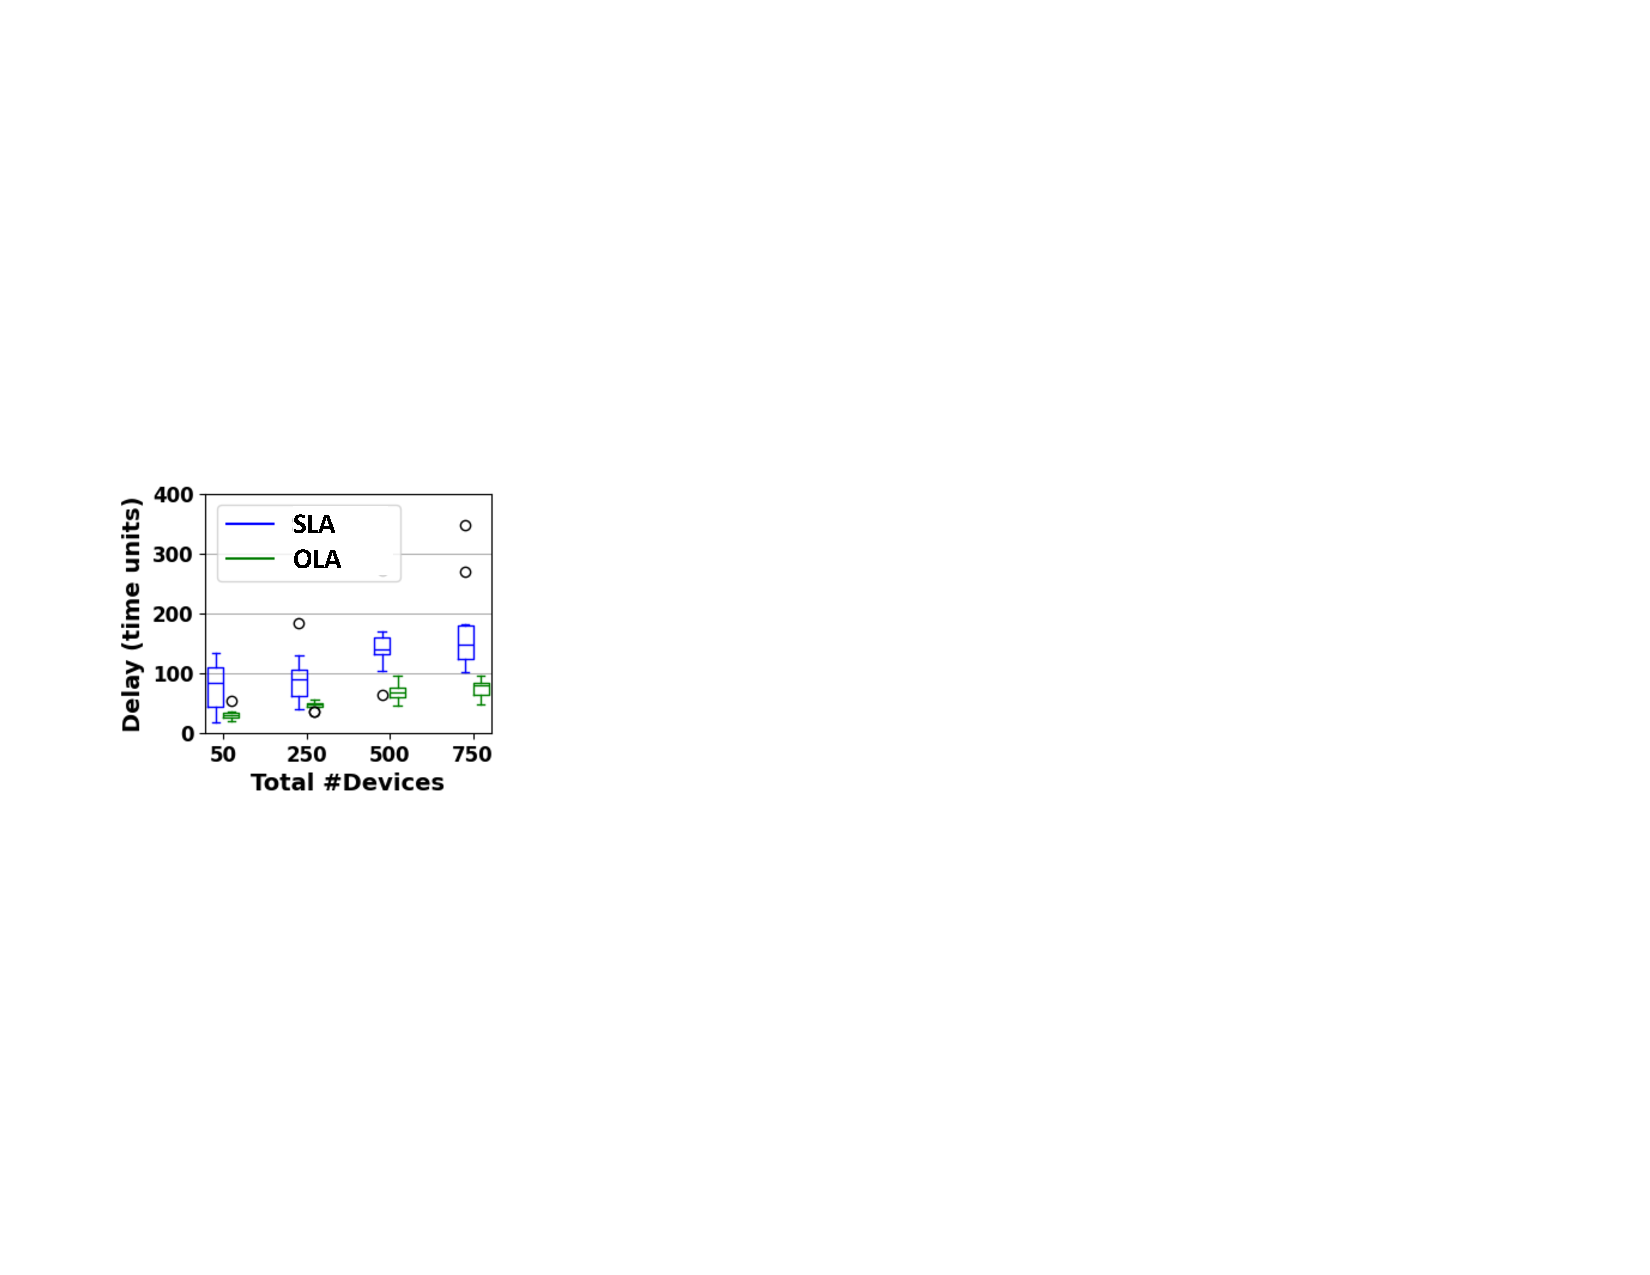
\includegraphics[width=\linewidth,alt={Grouped box-and-whisker plot for a grid topology. x-axis: total number of devices (50, 250, 500, 750); y-axis: delay in time units (0 to 400). Two series: SLA (blue) and OLA (green). OLA medians stay low (about 30 to 75) while SLA medians rise from about 85 to 150 as devices grow, so the optimistic strategy (OLA) consistently gives lower client delay than sequential (SLA).}]{CoMesh/figures/exp_eval/client_delay_cmp_grid_sla_vs_ola.pdf}
        \caption{\small \textit{Grid} topology.}
        \medskip
        \label{comesh:subfig:client_delay_grid}
    \end{subfigure}
    \hfill
    \begin{subfigure}[b]{0.31\linewidth}
        \centering
        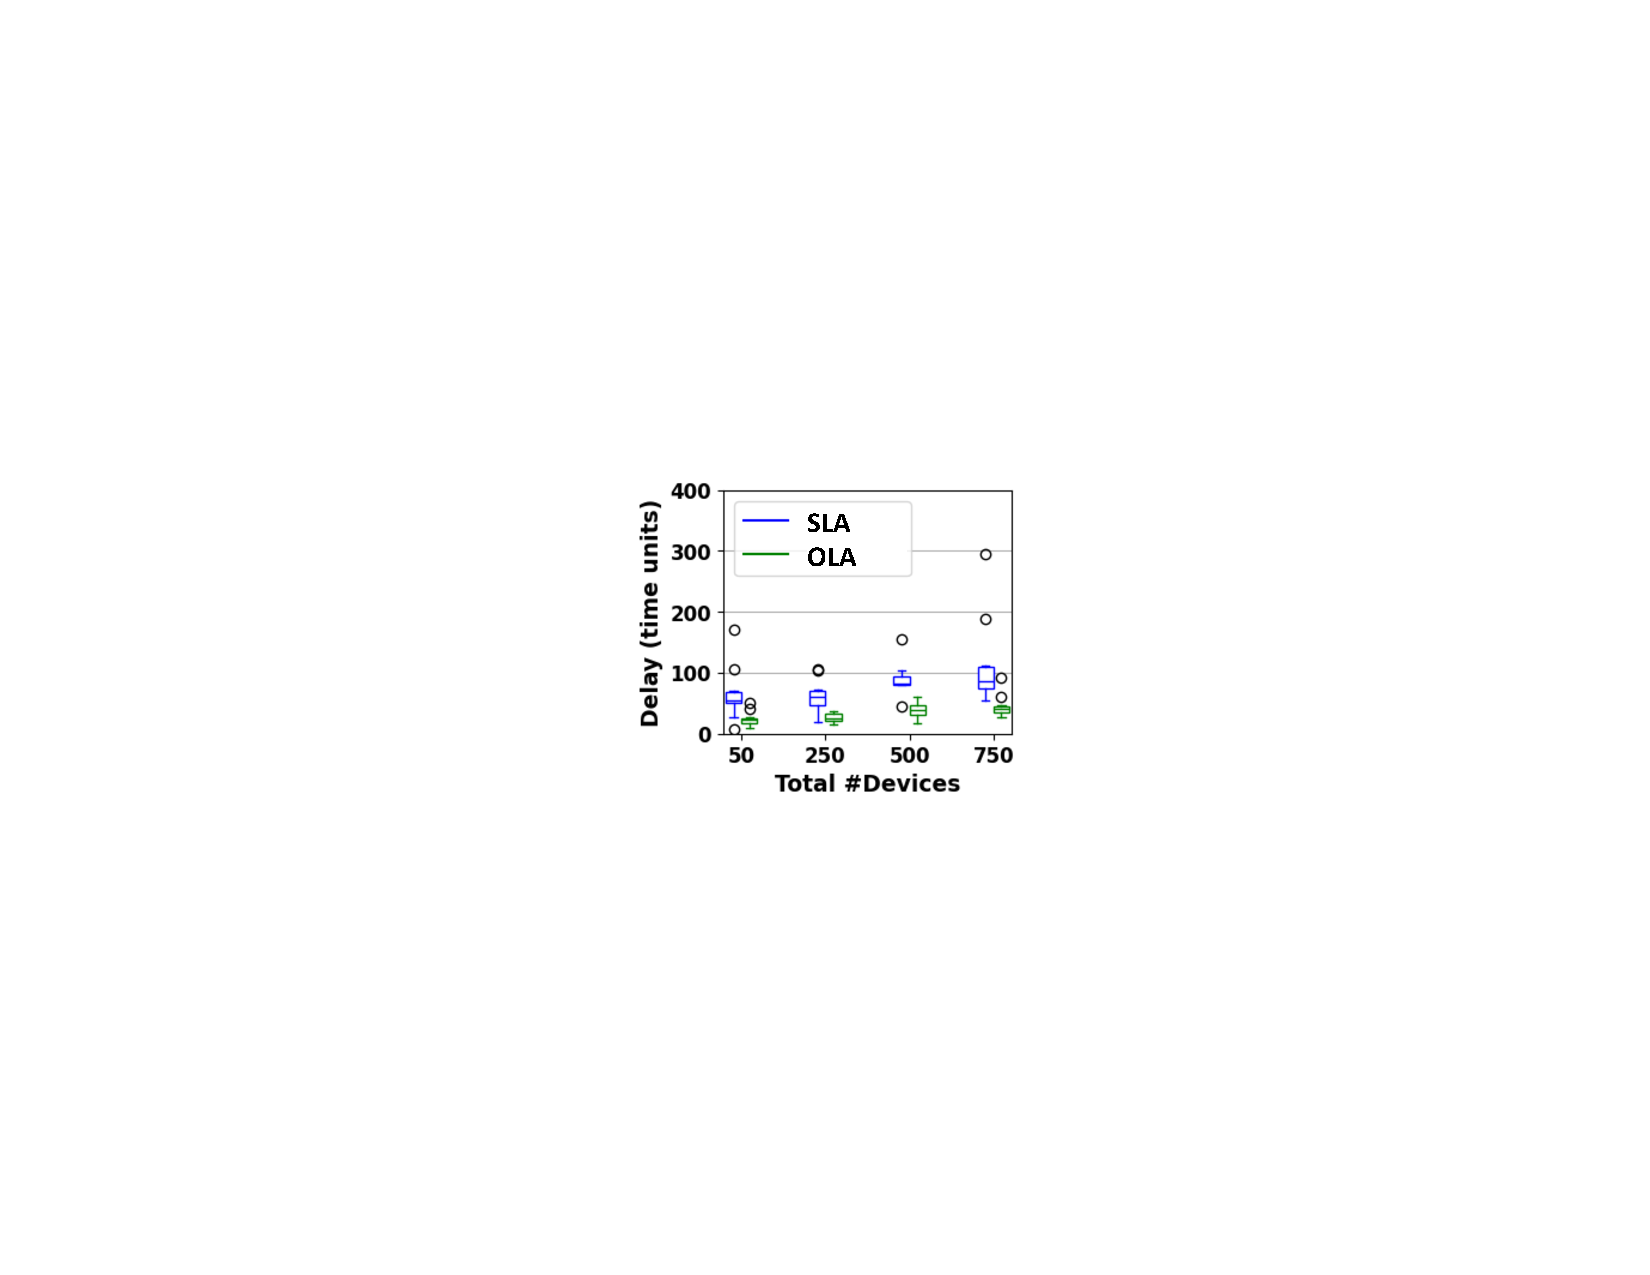
\includegraphics[width=\linewidth,alt={Grouped box-and-whisker plot for a random topology. x-axis: total number of devices (50, 250, 500, 750); y-axis: delay in time units (0 to 400). SLA (blue) medians rise from about 55 to 90 while OLA (green) medians stay around 20 to 42; OLA again gives consistently lower client delay than SLA.}]{CoMesh/figures/exp_eval/client_delay_cmp_random_sla_vs_ola.pdf}
        \caption{\small \textit{Random} topology.}
        \medskip
        \label{comesh:subfig:client_delay_random}
    \end{subfigure}
    \hfill
    \begin{subfigure}[b]{0.31\linewidth}
        \centering
        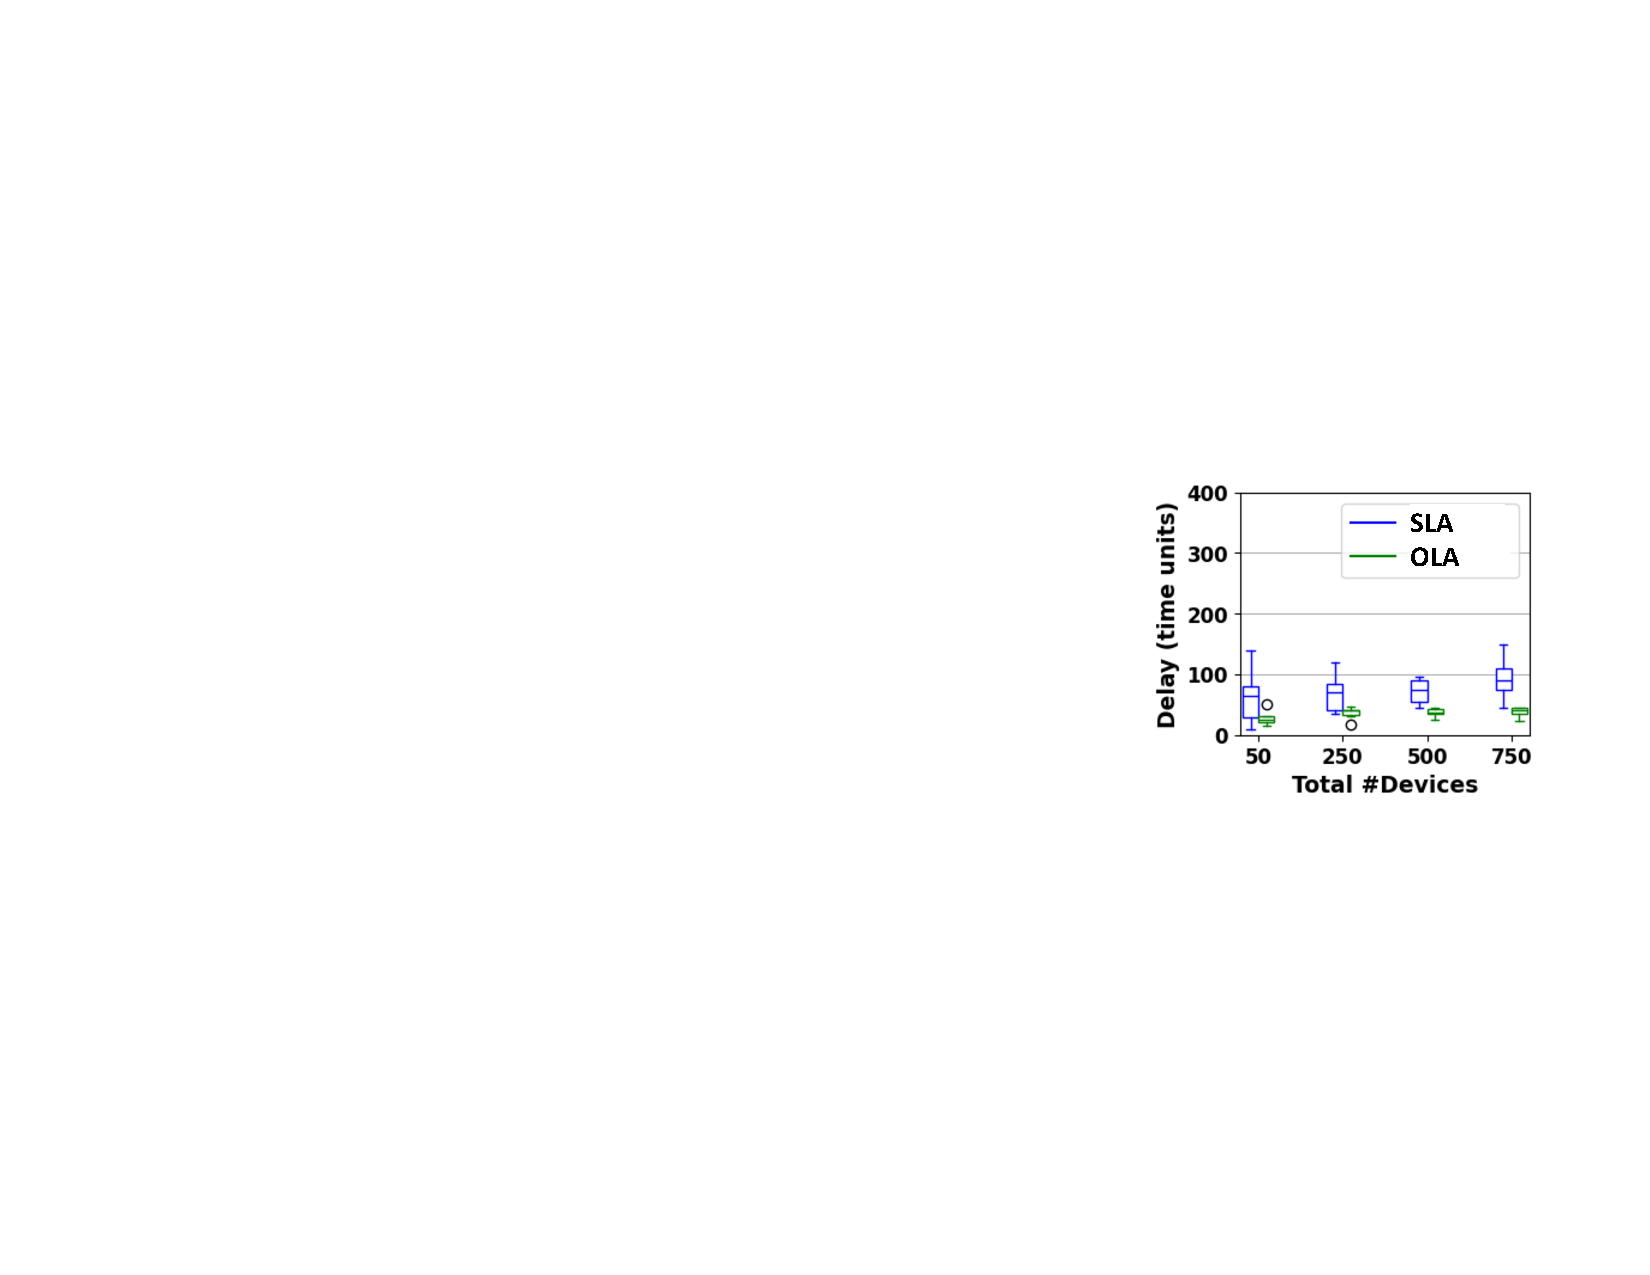
\includegraphics[width=\linewidth,alt={Grouped box-and-whisker plot for a clustered topology. x-axis: total number of devices (50, 250, 500, 750); y-axis: delay in time units (0 to 400). SLA (blue) medians rise from about 65 to 90 while OLA (green) medians stay stable around 25 to 40; OLA gives consistently lower client delay than SLA.}]{CoMesh/figures/exp_eval/client_delay_cmp_clustered_sla_vs_ola.pdf}
        \caption{\small \textit{Clustered} topology.}
        \medskip
        \label{comesh:subfig:client_delay_cluster}
    \end{subfigure}
    
    \caption{\small \it Client Delay: Sequential (SLA) vs. Optimistic (OLA) Lock-Acquiring Strategy, in three topologies.
    1 time unit is equivalent to 1 ms of real time.
    }
    \medskip
    \label{comesh:fig:pl-sr-comp}
\end{figure}

\begin{figure}[ht] % Use figure for spanning two columns in a two-column document
    \begin{minipage}{0.49\textwidth}
        \centering
        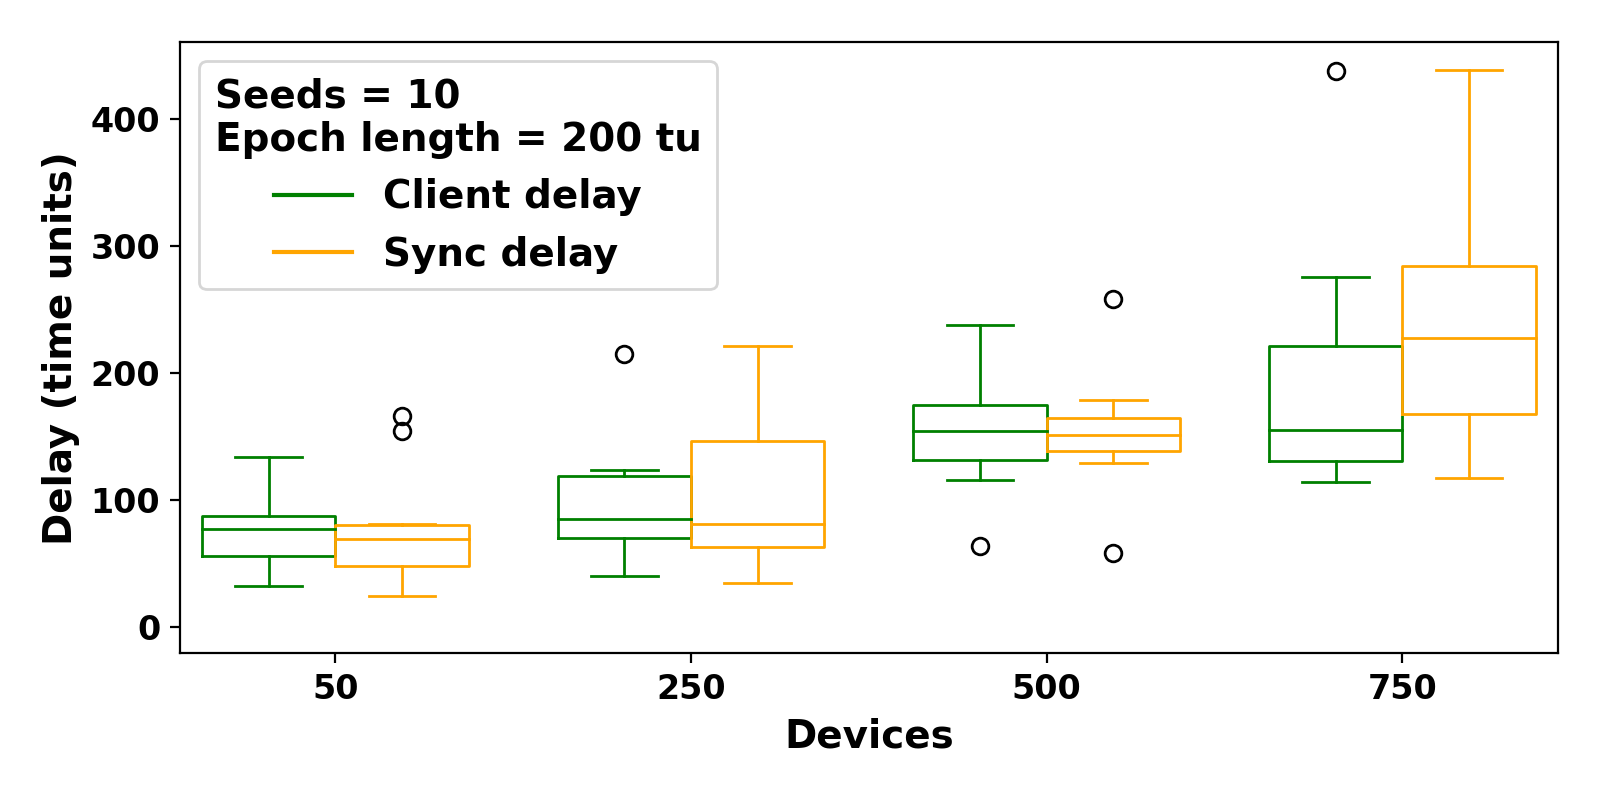
\includegraphics[width=\textwidth,alt={Grouped box-and-whisker plot for a grid topology with 40 percent device churn. x-axis: number of devices (50, 250, 500, 750); y-axis: delay in time units (0 to about 450). Two series: client delay (green) and sync delay (orange). Both medians rise with device count, from roughly 75 at 50 devices to about 155 (client) and 225 (sync) at 750 devices, with outliers above 400.}]{CoMesh/figures/exp_eval/client_sync_delays_failure_old.png}
        \caption{\small \it Client Delay
        and Sync Delay when 40\% of the \smart{}s in a grid topology experience churn (either a join or a failure).}
        \medskip
        \label{comesh:fig:client_sync_delay_failures}
    \end{minipage}
    \hfill
    \begin{minipage}{0.49\textwidth}
        \centering
        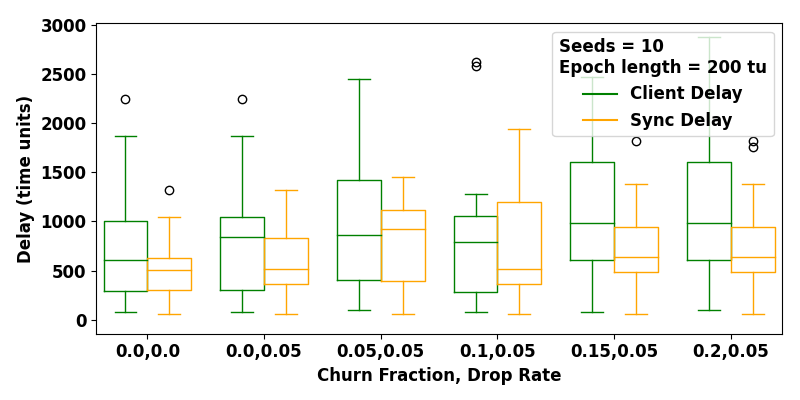
\includegraphics[width=\linewidth,alt={Grouped box-and-whisker plot. x-axis: churn fraction and packet drop rate pairs, from (0.0, 0.0) up to (0.2, 0.05); y-axis: delay in time units (0 to 3000). Two series: client delay (green) and sync delay (orange). Client-delay medians rise modestly from about 600 to about 1000 as churn increases, while sync-delay medians stay around 500 to 650; outliers reach about 2500.}]{CoMesh/figures/exp_eval/client_sync_delay_churn.png}
        \caption{\small \it Client and Sync Delays of routines under failure vs\. Churn fraction and packet Drop rate (80\% smart devices).}
        \medskip
        \label{comesh:fig:churn}
    \end{minipage}
\end{figure}

\noindent{\bf Client Delay.} 
Suppose there are no routines active. Then, if one routine's trigger conditions are activated, the time until executing its first command is the {\it client delay}---this measures a routine's cold-start time. Client delay  includes time for the routine \kgroup{} to
detect (and replicate) the trigger, lock all of its actuated devices, and start execution. 
In \Cref{comesh:fig:pl-sr-comp}, we observe that \sysname{}'s client delay scales (increases gently) with device count, regardless of topology or locking strategy.
As expected, optimistic locking (OLA) is faster than sequential locking (SLA) because client delay excludes conflicting routines. Among the 3 topologies, grid has higher client delay than random and clustered (which are similar), because the latter two have local density variations that form node ``clusters'' in the network which tend to speed up communication. Even though OLA is faster, we could prove liveness only for SLA~\cite{arxiv}. Users should employ OLA only in low-packet-drop networks, while SLA is robust, general-purpose, and still scalable. Scale goes up to 750 devices, similar to our dense smart building topology from \Cref{comesh:sec:mapsim}.

\noindent{\bf Churn Effect on Client/Sync Delays.} 
Churn refers to back-to-back smart device arrivals, departures, and failures. Even if membership lists are updated quickly (by underlying membership protocol Medley~\cite{medley}), \kgroup{} operations still incur overhead.
\Cref{comesh:fig:client_sync_delay_failures} shows that when 40\% of the \smart{}s  are churned 
in a grid topology (SLA locking),  client delay increases only 25\%, as some routines face the overhead of failover (election and state transfer).
To measure  \Cref{comesh:sec:pidep}'s  {\it sync delay},
we triggered two back-to-back instances of the identical routine.
{\Cref{comesh:fig:client_sync_delay_failures} shows  sync delay rises slowly---raising device count  by 15$\times$ from 50 to 750 causes $< 4 \times $ increase in sync delay (and client delay).} 
{Note that client delay does {\it not} subsume sync delay. 
Sync delay excludes triggering of routine and associated \kgroup{} quorum. Client delay excludes lock release latency and associated quorums. }

{
\noindent{\bf Effect of Stale Membership due to Drops and Churn.} 
{\it False detections} by the underlying membership may arise from dropped messages that make a failed device indistinguishable from a lossy one. This leads to inconsistent membership, and may slow \sysname's zero-message exchange mechanisms.
Yet, with 1000 devices and 80\% of them smart, \Cref{comesh:fig:churn} shows that raising packet drop rate (on all hops) from 0\%-5\%, along with churn fraction (\% smart devices failed during a run) keeps both client delay and sync delay stable.
Our churn and packet loss rates are much higher than in commercial deployments, which target 99.9\% uptime for devices~\cite{segarra2024uptime}. } 


\begin{figure}[tb!]
    \centering
    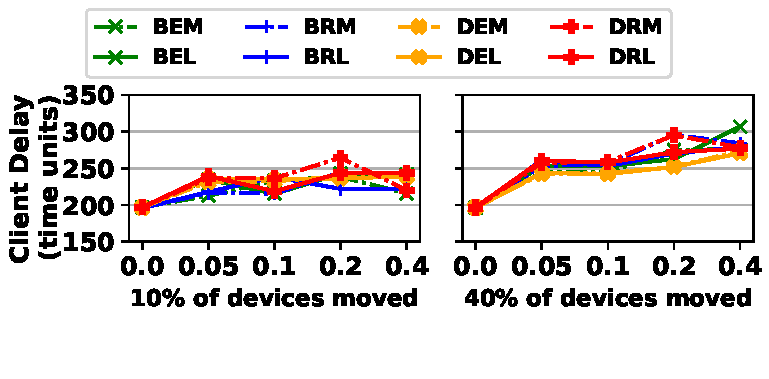
\includegraphics[width=0.6\linewidth,alt={Two side-by-side line subplots of client delay versus the maximum distance devices move (as a fraction of the topology dimension: 0.0, 0.05, 0.1, 0.2, 0.4); y-axis: client delay in time units (150 to 350). Eight series cover combinations of when mobility is injected (before or during epoch change or routine triggering) and whether the routine leader is included in the move. Left subplot (10 percent of devices moved): all curves start near 195 and rise modestly to about 220 to 265. Right subplot (40 percent moved): curves rise more steeply, reaching about 270 to 310 at the largest distance. Delay grows with both the fraction of devices moved and the distance moved.}]{CoMesh/figures/exp_eval/client_delay_wmobility.pdf}
    \caption{\small \it Mobility: Client delay vs. relative distance moved.
    }
    \medskip
    \label{comesh:fig:mobility}
\end{figure}

\noindent{\bf Device Mobility.}
\Cref{comesh:fig:mobility} shows the effect of device mobility, evaluated at different points of \sysname{} operation. With 250 devices organized in a $5 \times 5 \times 10$ grid, we instantly move a fraction of the devices, each randomly by distance in the interval $[0,X]$. After the instant move, routing 
tables are updated (for correct routing), but {\it we do not update the soft state of \sysname{} and keep it stale}.
\Cref{comesh:fig:mobility} shows 8 combinations created by injecting the mobility either at the start of or during a \sysname{} operation (B,D), during epoch change or routine triggering (E,R), and excluding or including routine leader (M,L). For space, we only plot client delay (sync delay showed similar behavior). We observe that with up to 10\% mobility \sysname{} raises client delay by less than 25\%. The degradation gets worse at higher mobility (40\%), but \sysname{} stays safe.
We conclude that \sysname{} can tolerate moderate mobility. 

\begin{figure}[tb!]
    \centering
    \begin{subfigure}[b]{0.4\linewidth}
        \centering
        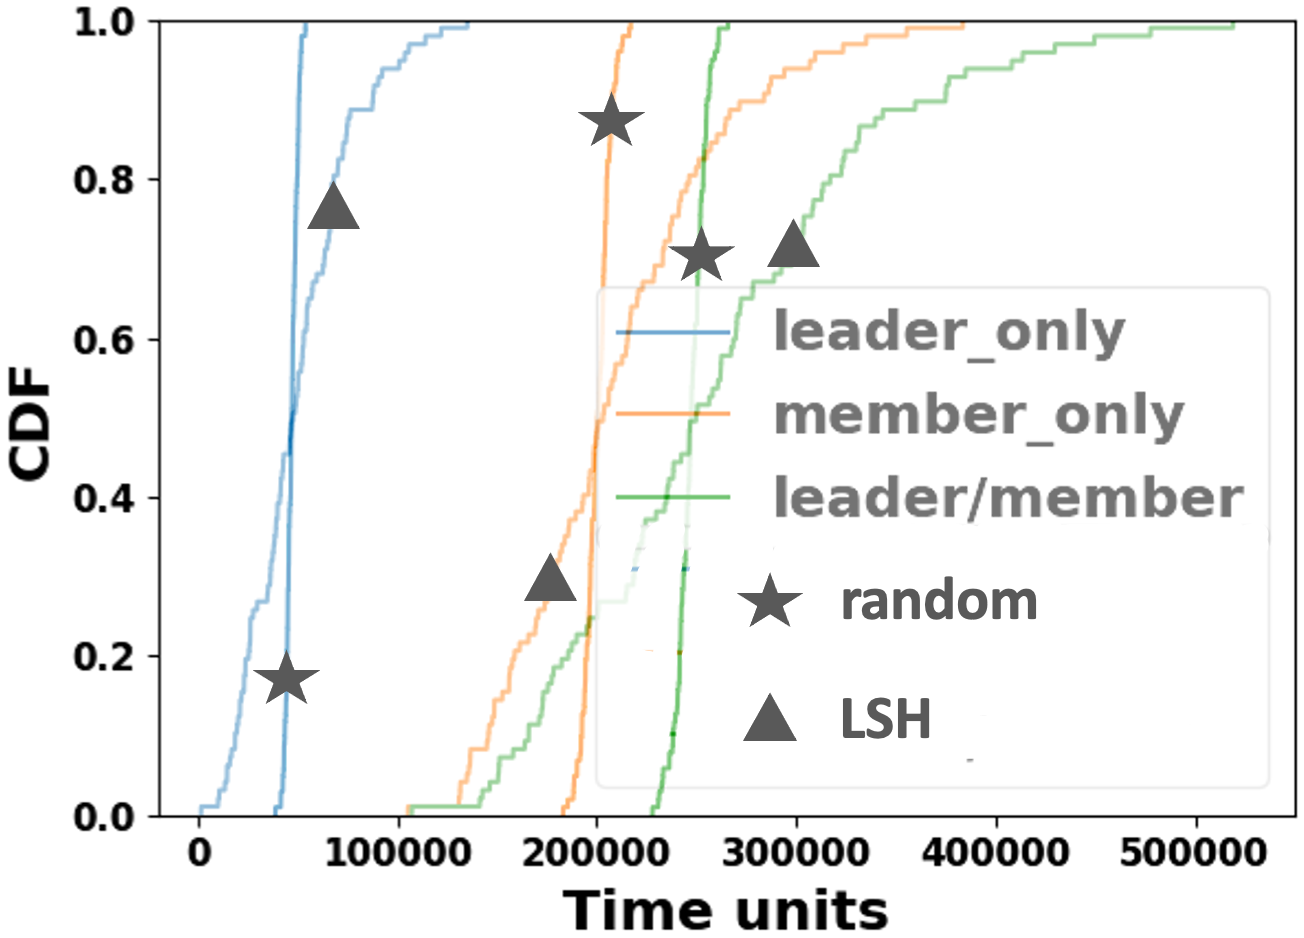
\includegraphics[width=\textwidth,alt={CDF plot. x-axis: temporal load in time units (0 to about 520,000); y-axis: cumulative probability (0 to 1). Three sets of curves curves by role: leader_only (blue, lowest load, roughly 0 to 130,000), member_only (orange, roughly 100,000 to 400,000), and leader/member (green, highest, roughly 150,000 to 520,000). Star markers denote the random policy and triangle markers the LSH policy; for each role LSH and random give similar median load but random is quite balanced across time whereas LSH is S-shaped, so LSH balances temporal load comparably to random despite a longer tail.}]{CoMesh/figures/exp_eval/temporal_load_balance_combined.png}
        \caption{\small \textit{Temporal} Load.}
        \medskip
        \label{comesh:subfig:temporal-load-balance-locality}
    \end{subfigure}
    \hspace{2cm}
    \begin{subfigure}[b]{0.4\linewidth}
        \centering
        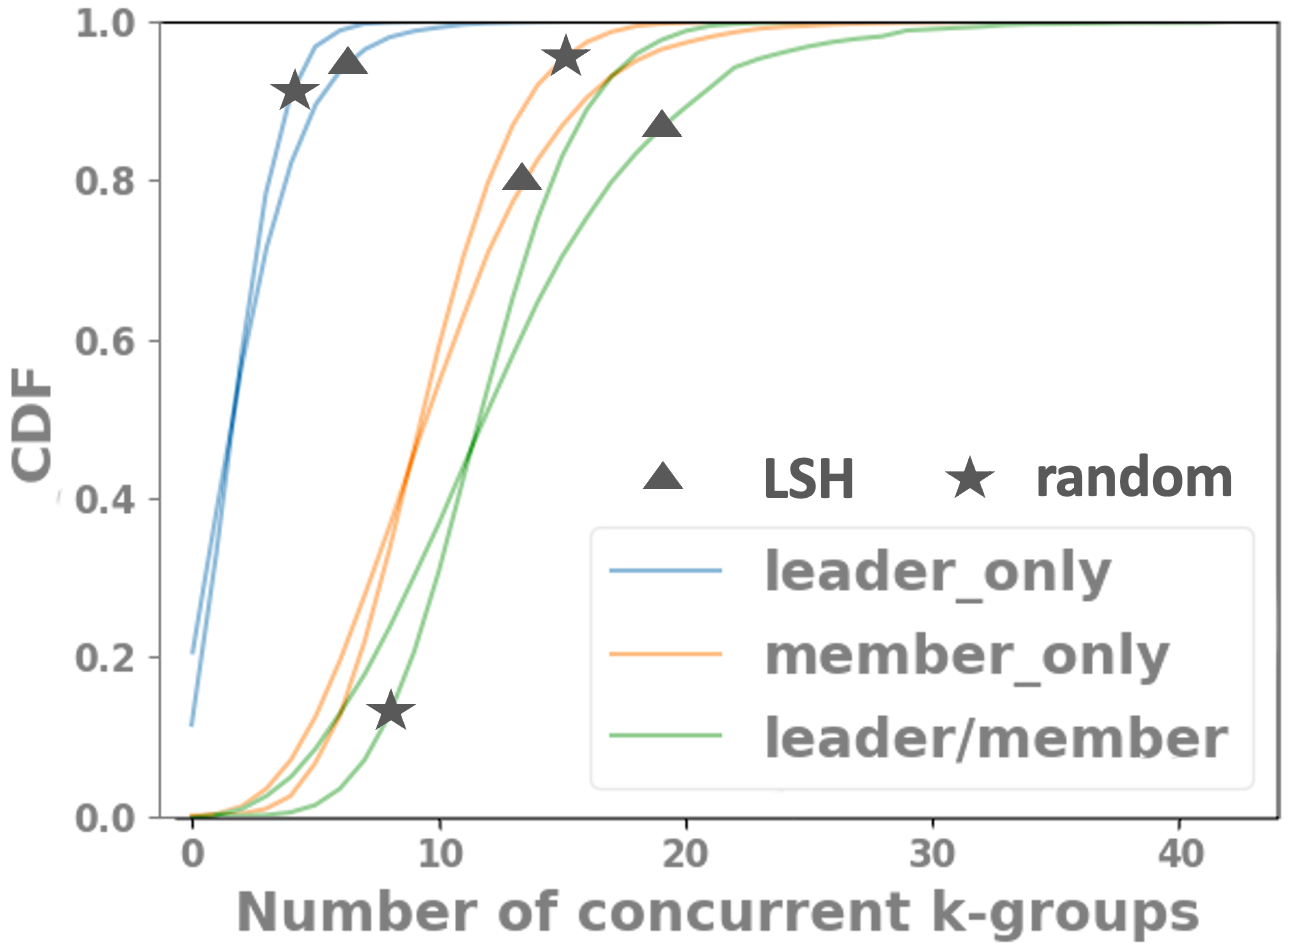
\includegraphics[width=\textwidth,alt={CDF plot. x-axis: number of concurrent \kgroups{} a device belongs to (0 to about 40); y-axis: cumulative probability (0 to 1). Three S-shaped sets of curves by role: leader_only (blue, lowest, about 0 to 7), member_only (orange, about 5 to 20), and leader/member (green, highest, about 5 to 25). Star markers mark the random policy and triangles the LSH policy; LSH and random track closely for each role, indicating comparable spatial load distribution.}]{CoMesh/figures/exp_eval/spatial_load_balance_combined.png}
        \caption{\small \textit{Spatial} Load.}
        \medskip
        \label{comesh:subfig:spatial-load-balance-locality}
    \end{subfigure}
    \caption{\small \it \sysname{}'s Load Distribution in Time \& Space: LSH/locality vs. Random (member \& leader selection). Grid topology.
    }
    \medskip
    \label{comesh:fig:load-balance}
\end{figure}

\noindent{\bf Load Distribution.} \Cref{comesh:fig:load-balance} measures two kinds of load distribution over a run:
{(1) {\it Temporal load} is the time that a smart device serves in a particular role.}
{(2) {\it Spatial load} is the number of concurrent \kgroups{}  a smart device is present in.}
{
The plots show LSH's clustering of \kgroups{} closer to target devices prolongs tail load vs. random due to repeated elections. Yet LSH's median temporal load for member and leader/member are similar to random's, showing LSH balances load well. 
}

\begin{figure}[ht]
    \centering
    \begin{minipage}{0.49\textwidth}
        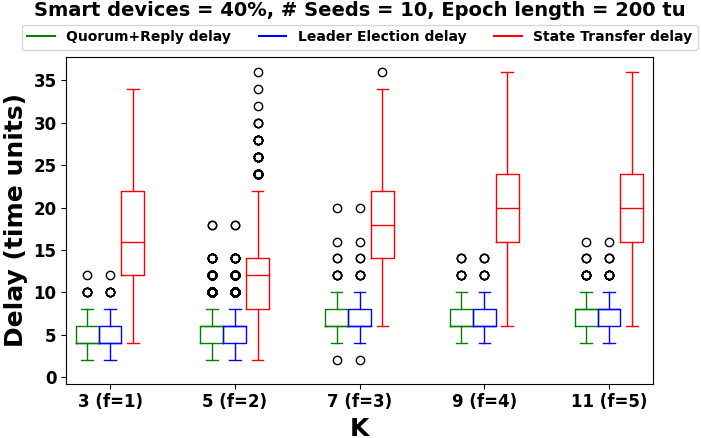
\includegraphics[width=0.99\textwidth,alt={Grouped box-and-whisker plot. x-axis: \kgroup{} size K from 3 (f=1) to 11 (f=5); y-axis: delay in time units (0 to about 36). Three series: quorum-plus-reply delay (green) and leader-election delay (blue), both low at about 5 to 7, and state-transfer delay (red), the highest, with medians rising from about 16 to 20 as K grows. Within-\kgroup{} delay is dominated by state transfer and increases with K.}]{CoMesh/figures/exp_eval/in_kgroup_variable_k_smaller.png}
        \caption{\small \it Delays of operations within a \Kgroup{} for different $\K$.\\}
        \medskip
        \label{comesh:fig:in_kgroup_ks}
    \end{minipage}
    \hfill
    \begin{minipage}{0.49\textwidth}
        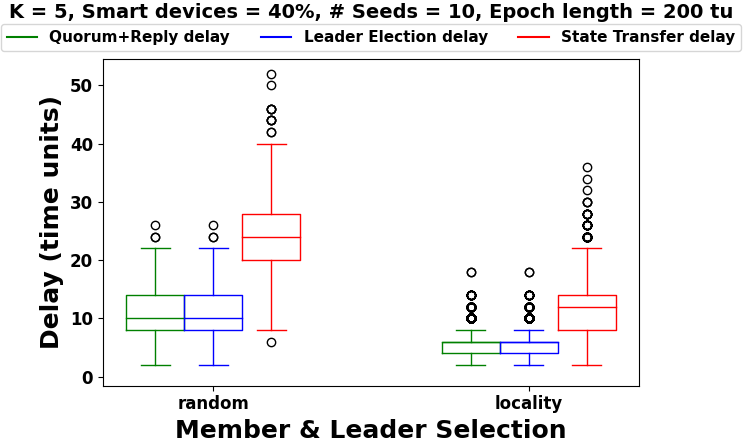
\includegraphics[width=1.02\textwidth,alt={Grouped box-and-whisker plot comparing two selection policies (K=5). x-axis: member and leader selection (random vs locality); y-axis: delay in time units (0 to about 52). Three series: quorum-plus-reply (green), leader-election (blue), and state-transfer (red) delay. Under random selection medians are about 10 (green and blue) and 24 (red); under locality they drop to about 5 and 12, so locality-based selection roughly halves all three delays.}]{CoMesh/figures/exp_eval/in_kgroup_policies_new.png}
        \caption{\small \it Delays of operations within a \Kgroup{} for different policies of entity clustering, member selection, and leader election.}
        \medskip
        \label{comesh:fig:in_kgroup_policies}
    \end{minipage}
    \begin{minipage}{\textwidth}
        \vspace{0.5cm}
        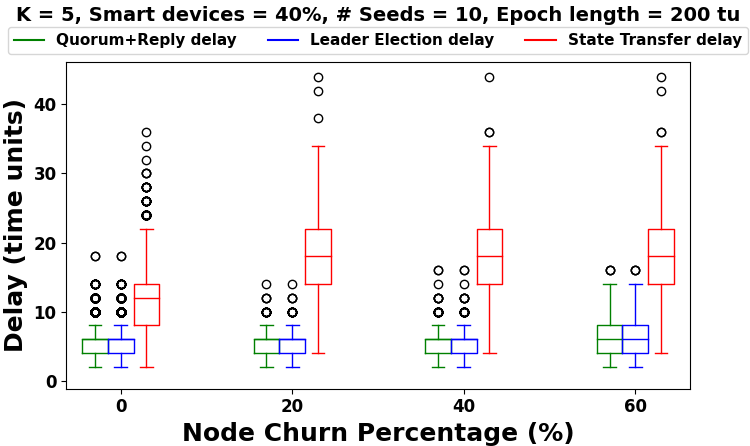
\includegraphics[width=0.5\textwidth,alt={Grouped box-and-whisker plot (K=5). x-axis: node churn percentage (0, 20, 40, 60); y-axis: delay in time units (0 to about 44). Three series: quorum-plus-reply (green) and leader-election (blue) delay stay low and flat at about 5 to 6 across all churn levels, while state-transfer delay (red) rises from about 12 at no churn to about 18 to 20 once churn is present and then stays flat, so within-\kgroup{} operations are largely robust to churn.}]{CoMesh/figures/exp_eval/in_kgroup_wf_smaller.png}
        \caption{\small \it \Kgroup{} Internal Operations vs. Smart Device  Churn.\\}
        \medskip
        \label{comesh:fig:in_kgroup_failure}
    \end{minipage}
\end{figure}

\noindent{\bf {\Kgroup{} Operations}.}
\Cref{comesh:fig:in_kgroup_ks}  measures \kgroup{} internal performance (default parameters:   \Cref{comesh:tab:def_param_vals}). All \kgroup{} operations---election, quorum,  state transfer---scale   as \kgroup{} size is increased from 3 ($f=1$) to 11 ($f=5$). Quorums are scalable because requests and replies are sent in parallel. Leader election delays are scalable as the Bully algorithm is fast in the common case.
State transfer delay is a function of the amount of state, but does not depend on coterie size $k$.

\Cref{comesh:fig:in_kgroup_policies} confirms our hypothesis that locality-awareness (LSH of  (\Cref{comesh:subsection:lsh})) 
decreases operational delays of a \kgroup{}. The improvement from LSH is more prominent for election and quorum due to the localized communication (state transfer is dominated by the old leader to new leader bandwidth). 

\Cref{comesh:fig:in_kgroup_failure} shows  a \kgroup's  operations are not 
affected by churn among \smarts, except beyond 60\% churn. Essentially, requiring only a quorum imbues churn-tolerance. When $\f$ members fail, the \kgroup's leader recruits replacements to tolerate future failures (\Cref{comesh:subsection:fault-tolerance}). 

\subsubsection{Map-Driven Simulation with Real Workloads}
\label{comesh:sec:mapsim}

We perform a large simulation using a real building map and a realistic routine workload mix. 
{The \Bldg{} (\Cref{comesh:fig:IoTsetting}(a)) is a ``living laboratory'' sized 250 ft $\times$ 362 ft, with
sensors and actuators in offices, lecture halls, and conference rooms. 
Map-driven simulation allows us to flexibly vary device densities, transmission radii, and routine sets.
Our simulator (\Cref{comesh:sec:simres}) includes this map with two topologies: 
(i) a {\it \largeT{}} topology with 708 devices, and (ii) a {\it \smallT{}} topology with 285 devices. \LargeT{} topology has 4.06 $\pm$ 2.31 devices per room \& corridor. \SmallT{} topology has 3.43 $\pm$ 1.79. 40\% of devices are smart.
\SmallT{}  has motion sensors and lights, while  \largeT{}  also has thermostats, light sensors, shades, and microphones.

\begin{figure}[tb!]
    \centering
    \begin{subfigure}[b]{0.4\linewidth}
        \centering
        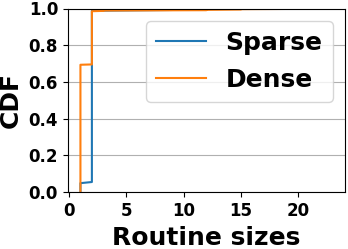
\includegraphics[width=0.775\textwidth,alt={CDF plot. x-axis: routine size, i.e., the number of devices a routine actuates (0 to 22); y-axis: cumulative probability (0 to 1). Two step curves: Sparse (blue) and Dense (orange) topologies. Both reach close to 1.0 by a routine size of 2, with the Dense curve already near 0.7 at size 1, so almost all routines actuate just one or two devices and very few are larger.}]{CoMesh/figures/exp_eval/rtn_sizes.png}
        \caption{\small \it CDF of how many devices a routine actuates. 
        }
        \medskip
        \label{comesh:subfig:rtn_sizes}
    \end{subfigure}
    \hfill
    \begin{subfigure}[b]{0.57\linewidth}
        \centering
        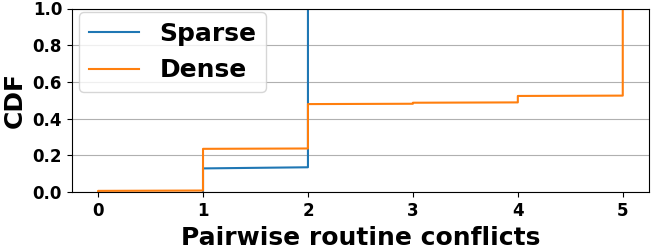
\includegraphics[width=\textwidth,alt={CDF plot. x-axis: number of pairwise routine conflicts (0 to 5); y-axis: cumulative probability (0 to 1). Two step curves: Sparse (blue) reaches 1.0 by 2 conflicts, while Dense (orange) climbs to about 0.5 by 2 conflicts and then has a long tail, reaching 1.0 only at 5. The dense topology produces more conflicting routine pairs than the sparse one.}]{CoMesh/figures/exp_eval/rtn_conflicts.png}
        \caption{\small \it CDF of the number of conflicting actuated devices between routine pairs.
        }
        \medskip
        \label{comesh:subfig:rtn_conflicts_cdf}
    \end{subfigure}
    \par\medskip
    \begin{subfigure}[b]{\linewidth}
        \centering
        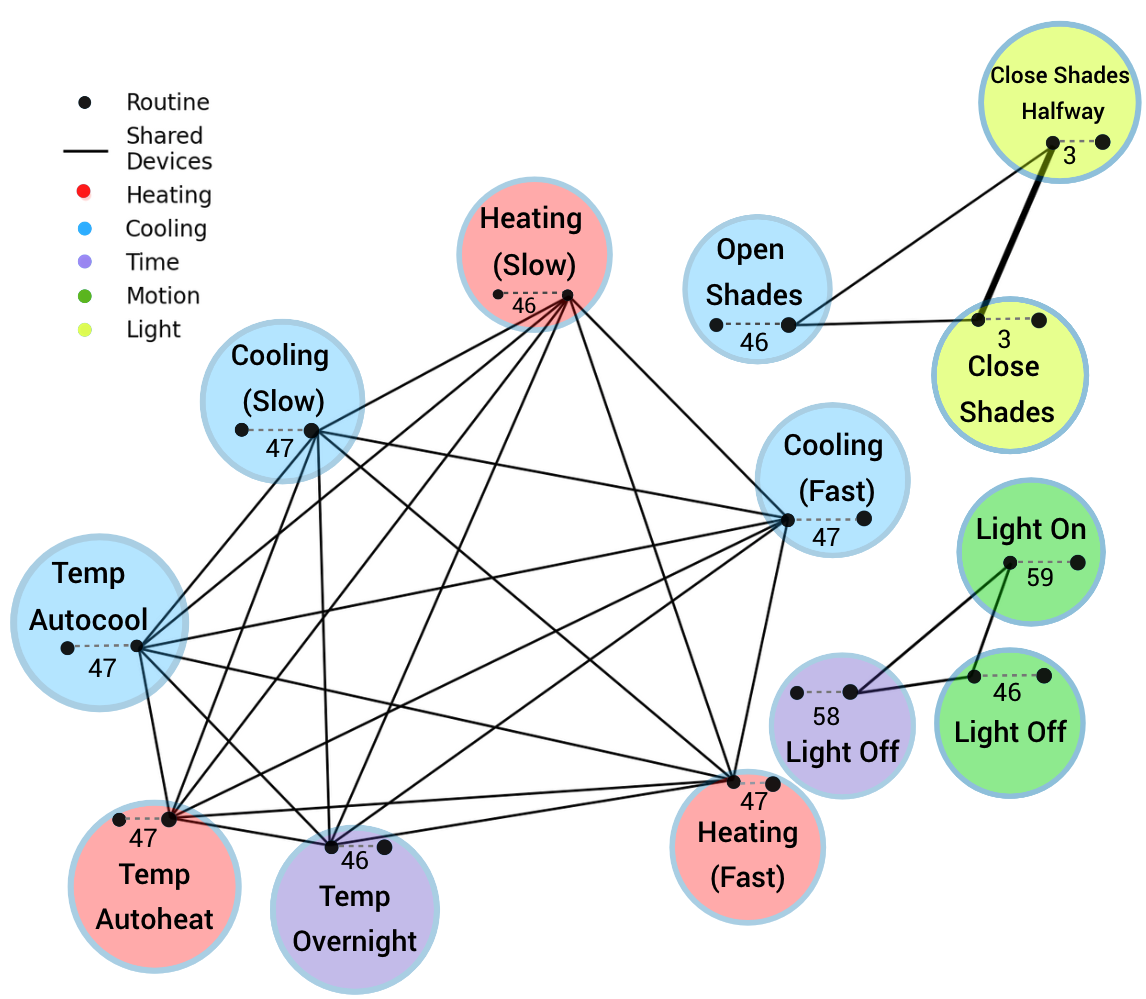
\includegraphics[width=0.9\linewidth,alt={Node-link graph of routine conflict classes. Each node is a circle whose color encodes trigger condition: red for heating, blue for cooling, purple for time, green for motion, and light green for light. Labeled nodes include Heating (Slow): 46 routines, Open Shades: 46, Cooling (Fast): 47, Light On: 59, Light Off based on motion: 46, Light Off based on time: 58, Heating (Fast): 47, Temp Overnight: 46, Temp Autoheat: 47, Temp Autocool: 47, Cooling (Slow): 47, Close Shades: 3, Close Shades Halfway: 3. Edges connect classes that share conflicting devices; the thicker the edge the more conflicting devices between those two classes. The graph is dense in the center around the heatinga and cooling classes, and sparser at the periphery for small-routine classes around shades and lights classes.}]{CoMesh/figures/exp_eval/rtn_conflict_graph.png}
        \caption{\small \it Routine conflicts for the \SmallT{} (bottom right 3 classes) and \LargeT{} topologies. Circle = routine class; Color = trigger condition; Count = number of routines; Thicker edges = more conflicting devices.   
        }
        \medskip
        \label{comesh:fig:rtn_conflicts}
    \end{subfigure}
    \caption{\small \it Workload in 
    \Bldg{} Map-Driven Simulations. \LargeT{} topology: all 545 routines. 
    \SmallT{} topology: 163 routines. 
    }
    \medskip
    \label{comesh:fig:rtn_stats}
\end{figure}

We created a routine workload mix based on devices and frequently observed actions
from this building.  \Cref{comesh:fig:rtn_stats}(a,b) show a CDF of device count actuated by a routine, and pairwise routine conflicts. 
\Cref{comesh:fig:rtn_conflicts} shows major routine classes (only 2 representatives shown out of many), and typical conflicts. 
The \largeT{} (respectively \smallT{}) topology has 545 active routines (resp. 163),
containing 1-23 commands with mean  1.47 and median 1  (resp. for \smallT: 1-12, median: 2, mean: 2.07). 
We calibrated the simulator so that  
1 time unit in the simulation is equivalent to 1 ms of real time. Based on our measurements of inter-Raspberry Pi latencies, we set the hop latency realistically to $(1.4 \times e^{(0.03 \cdot distance)})$ ms.
}

\begin{figure}[th!]
    \centering
    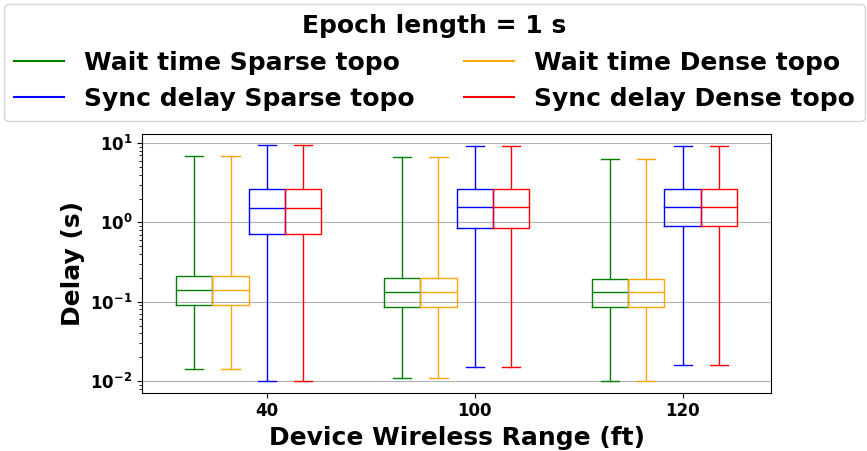
\includegraphics[scale=0.5,alt={Grouped box-and-whisker plot with a logarithmic y-axis. x-axis: device wireless range in feet (40, 100, 120); y-axis: delay in seconds (about 0.01 to 10). Four series: wait time for sparse (green) and dense (orange) topologies, and sync delay for sparse (blue) and dense (red) topologies. Wait-time medians are low at about 0.1 to 0.15 seconds while sync-delay medians are higher at about 1 to 1.5 seconds; all stay roughly flat across the three wireless ranges.}]{CoMesh/figures/exp_eval/client_sync_delay_comparison_logy.png}
    \caption{\small \it \Bldg{} (Map-driven) Simulation (\Cref{comesh:fig:IoTsetting}(a)): Wait times and Sync delays vs. device transmission range. (1 time unit in simulation $\simeq$ 1 ms of real time). Upper end shows max. 
    }
    \medskip
    \label{comesh:fig:siebel_delays}
\end{figure}

\Cref{comesh:fig:siebel_delays}  shows Sync delay and Wait time. Sync delay is the handover time from one finishing routine to the next waiting routine (same as \Cref{comesh:sec:pidep}). {\it Wait time} is the time from when a routine is triggered until it executes its first command---this metric measures \sysname's overheads that may delay the start of a routine after it is triggered. 
With a sparse topology (40 ft transmission range),  wait time is 0.22 s at median (2.55 s max), while sync delay (handover time from routine to routine) is 1.76 s at median (8.89 s max). For \largeT{} topology, wait time median is 0.14 s, and sync time median is 1.5 s. Higher transmission ranges of 100 ft and 120 ft only slightly decrease these metrics, e.g., for \smallT{} topology,
wait time medians are 0.2 s and 0.2 s respectively, and sync delay medians are 1.7 s and 1.62 s respectively. We conclude that   \sysname{} scales well in a real building under a real routine workload. 

